\documentclass[11pt]{article}
\usepackage[margin=1in,includefoot]{geometry}

\usepackage{color}
\usepackage{tikz}
\usepackage{mathtools}
\usepackage{mathpartir}
\usepackage{amsmath}
\usepackage{amssymb}
\usepackage{url}
%\usepackage{bnf}
\usepackage{local}
\usepackage{xspace}
\usepackage{graphicx}
\graphicspath{ {images/} }
\usepackage{fancyvrb}
\usepackage[margin=1in]{geometry}

\usepackage{listings}
\usepackage{balance}

\lstset{
  basicstyle=\footnotesize\ttfamily,
  breaklines=true,
  frame=none,
  language=haskell,
  %identifierstyle=\color{identifierColor},
  backgroundcolor=\color{white},   % choose the background color; you must add \usepackage{color} or \usepackage{xcolor}
  breakatwhitespace=false,         % sets if automatic breaks should only happen at whitespace
  %captionpos=b,                    % sets the caption-position to bottom
  %commentstyle=\color{mygreen},    % comment style
  %frame=single,	                   % adds a frame around the code
  keepspaces=true,                 % keeps spaces in text, useful for keeping indentation of code (possibly needs columns=flexible)
  keywordstyle=\color{blue},       % keyword style
  otherkeywords={*,let, Server, Replication, FaultGraph, rankRCG, print, fialProb, goal, ...},           % if you want to add more keywords to the set
  numbers=none,                    % where to put the line-numbers; possible values are (none, left, right)
  numbersep=5pt,                   % how far the line-numbers are from the code
  rulecolor=\color{black},         % if not set, the frame-color may be changed on line-breaks within not-black text (e.g. comments (green here))
  showtabs=false,                  % show tabs within strings adding particular underscores
  stepnumber=1,                    % the step between two line-numbers. If it's 1, each line will be numbered
  %title=\lstname                  % show the filename of files included with \lstinputlisting; also try caption instead of title
  mathescape=true,
  tabsize=3,
  literate=*{->}{{\textcolor{blue}{$\to$}}}{1}
           {<-}{{\textcolor{blue}{$\leftarrow$}}}{1}
}




\begin{document}
\renewcommand\t[1]{\texttt{#1}}
\newcommand\base{\alpha} % Base data-type
\newcommand\todo[1]{{\color{red}#1}}
\newcommand\where{\;|\;}
\newcommand\bnfalt{\;\;|\;\;}
\newcommand\bnfas{\;:=\;}

\newcommand\set{S}
\newcommand\elt{s} % element of a set
\newcommand\func{F} % Function

\newcommand\true{$\t{true}$}
\newcommand\false{$\t{false}$}

\newcommand\val{v} % atomic value
\newcommand\expr{e} % Expression
\newcommand\inp{I} % input
\newcommand\var{x} % variable

\newcommand\sem[1]{[\![#1]\!]}


\def\widowpage{\pagebreak}

% Choose abbreviated or long-version alternatives in paper
%\long\def\abbr#1#2{#1}			% abbreviated version
\long\def\abbr#1#2{#2}			% long version

% Choose abbreviations or long names/titles in bibliography
%\def\bibbrev#1#2{#1}			% short version
%\def\bibbrev#1#2{#2}			% long version
\def\bibbrev#1#2{\abbr{#1}{#2}}		% follow abbr macro

% Abbreviated or full citation lists: \abcite{basic}{others}
\newcommand{\abcite}[2]{\abbr{\cite{#1}}{\cite{#1,#2}}}

% Conference abbreviations: \bibconf[Nth]{SOSP}{Symposium on ...}
\newcommand{\bibconf}[3][]{#1 \bibbrev{#2}{#3 (#2)}}

\newcommand{\ie}{{\em i.e.\xspace}}
\newcommand{\eg}{{\em e.g.\xspace}}

% system related terms
\newcommand{\app}{ConfigV\xspace}

\long\def\com#1{}

\long\def\ennan#1{{\color{blue}{\bf Ennan: }{\small [#1]}}}
\long\def\ruzica#1{{\color{red}{\bf Ruzica: }{\small [#1]}}}

\newcommand{\para}[1]{\smallskip\noindent {\bf #1}}


%\section*{Cooperative Programming: Integrating Software Synthesis with the Live Paradigm}
\paragraph{Overview:} Live programming is an emerging paradigm that is promising a vast change in the techniques used to develop modern software. A live programming environment allows a programmer to immediately see the effects of changes to a program on its outputs and effectively eliminates the edit-run-debug cycle that dominates programming workflows today. Our work seeks to develop new synthesis techniques that make use of the real-time feedback loop provided by a live programming environment. We will develop a system that allows a user to track a set of examples and synthesize subroutines to fit that set. When combined with fault localization techniques, programmers will be able to quickly find incorrect sections of code and initiate repairs that leverage information gleaned from the provided examples. While current  development tools provide tangible benefits to programmers skilled enough to use them, we aim to develop an accessible, first-of-its-kind, \textit{cooperative programming} environment that provides feedback in the form of generating representative examples and allowing changes to the code to be made through adjustments to these examples.

\paragraph{Intellectual Merits:} There are several open-ended problems that will be explored as a part of this research. In particular, we will need to:

\begin{itemize}
\item Create novel, real-time algorithms to synthesize code within a live programming environment.
\item Investigate methods to evaluate the quality of an example set and methods to produce high quality example sets for a given program.
\item Build a formal theoretical framework for synthesis in a feedback loop.
\item Integrate these developments in a unified environment for a modern, major programming language - namely, Haskell.
\end{itemize}

\paragraph{Broader Impact:} We believe that cooperative programming environments will increase programmer productivity while simultaneously lowering the barriers for entry for newcomers to computer programming. As we develop the theory behind the techniques needed to realize this environment, the our approach will be informed by the needs of programmers, for whom these systems are ultimately built. We will publish our theoretical developments, open source our code, and maintain the tools we produce to foster community involvement while at the same time visiting universities, industrial labs, and top conferences to gain collaborators and share our work with fellow researchers in the field.

In addition to our proposed theoretical developments, we aim to introduce our environment to novice programmers in secondary educational programs. We have promised support from the Connecticut Computer Science Teachers Association, and we are excited to work with them to build a cooperative programming environment that is approachable and useful to beginner and expert programmers alike.


\newpage
\pagenumbering{arabic}
\setcounter{page}{1}

\section{Motivation}
\label{sec:intro}

Configuration errors are one of the most important root causes of
today's software system failures~\cite{xu15systems, yin11anempirical}.
Recently, there was a problem in accessing  
Facebook and Instagram~\cite{mashableNews}, 
and a Facebook spokeswoman reported that 
this was caused by a change to the site's configuration systems.
In a recent software system failures study~\cite{yin11anempirical},
researchers revealed that about 31\% of system failures were caused by 
configuration errors, which is higher than the percentage of
failures resulting from program bugs (20\%). 
%(which and only 20\% were caused by bugs in program code 
%While program verification is mostly focused on detecting errors 
%in code, in their empirical study 
%Yin {\em et al.}~\cite{yin11anempirical} report
%that about 31\% of system failures were caused by configuration errors problems and only 20\% were caused by bugs in program code. 
Configuration errors are commonly referred to in the literature 
as misconfigurations. 

Misconfigurations, in practice, may result in various
system-wide problems, such as security vulnerabilities, 
application crashes, severe disruptions in software
functionality, and incorrect program executions%
~\cite{zhang14encore, yuan11context, xu13do, xu15hey}. 

The systems research community has recognized this as an important
problem. In fact, at this year's OSDI conference (Operating Systems
Design and Implementation, a top-tier system conference) a paper on
detecting configuration errors by emulating the late execution
 ~\cite{xu16early} received the best paper 
award. While many efforts have been proposed to check, troubleshoot, diagnose, and repair configuration errors~\cite{attariyan10automating,
su07autobash, whitaker04configuration},
those tools mainly try to understand {\emph{what}} caused the 
error -- they are still not on a level of
automatic verification tools used for regular program 
verification~\cite{Leino10Dafny, PiskacWZ14, BobotFMP15} that can
detect errors without executing the code. Our proposal offers 
automated verification of configuration files: we are analyzing 
files and proactively reporting potential errors, without waiting for them to happen.

\subsection{Examples}
\label{sec:intro-examples}

We start by presenting two non-trivial configuration errors
extracted from real-world examples. 
Although the errors are relatively simple, we call them 
non-trivial, because the majority of existing misconfiguration
checking tools~\cite{zhang14encore, wang04automatic} cannot detect
these configuration errors. 
Most of the presented examples were found on
StackOverflow~\cite{stackoverflow},
a popular Q\&A website for programmers.

\para{Example~1: Ordering errors.} 
When a user configures PHP  to run with the Apache HTTP Server, most 
likely the user will take some already existing configuration files and 
adapt them to suit her needs. The configuration file might contain, among 
others,  the following lines:
\begin{lstlisting}[language=C, xleftmargin=.01\textwidth]
extension = mysql.so
...
extension = recode.so
\end{lstlisting} 
In this case, the configuration file will cause the Apache server to 
fail to start due to a segmentation fault error. 
This is because, when using PHP in Apache, the extension {\tt mysql.so} 
depends on {\tt recode.so}, and their relative ordering
is crucial. This is an example of an {\em ordering error}.
Yin {\em et al.} report that ordering errors widely exist in
many system configurations, \eg, PHP and MySQL,
and typically lead to multiple system crash events.
However, no existing tool in the systems research area can effectively solve 
or detect this problem~\cite{zhang14encore, xu15systems, xu13do}.


\para{Example~2: Fine-grained value correlation error.} 
Our next example also comes from a discussion on 
StackOverflow~\cite{correlation}.
The user has configured her MySQL as follows:
\begin{lstlisting}[language=C, xleftmargin=.01\textwidth]
key_buffer_size = 384M
max_heap_table_size = 128M
max_connections = 64
thread_cache_size = 8
...
sort_buffer_size = 32M
join_buffer_size = 32M
read_buffer_size = 32M
read_rnd_buffer_size = 8M
...
\end{lstlisting} 
The user complained that her MySQL load was very high, causing the website's
response speed to be very slow.
In this case, {\tt key\_buffer\_size} is used by all the threads
cooperatively, while {\tt join\_buffer} and {\tt sort\_buffer} are 
created by each thread for private use; thus, the maximum amount
of used key buffer, \ie, {\tt key\_buffer\_size}, should be larger than 
{\tt join|sort\_buffer\_size} * {\tt max\_connections}. 
Clearly, in the above example, this does not hold, 
so this misconfiguration causes MySQL to load very slowly.
This type of error is more sophisticated than the simple value correlation that some tools can detect~\cite{yin11anempirical, zhang14encore}.


\subsection{Challenges}
\label{sec:intro-chal}

We believe there are two main obstacles 
to simply applying the existing automatic 
tools and techniques to verification of configuration files:
\begin{itemize}
\item the lack
of a specification describing properties of configuration files
\item the structure of configuration files -- they
are mainly a sequence of entries assigning some value to system
variables (called {\emph {keywords}}). 
\end{itemize}
The language in which configuration files are written does 
not adhere to a specific grammar or syntax. In particular, the
entries in configuration files are untyped. Moreover, there are surprisingly few rules specifying constraints on entries, and there
is no explicit structure policy for the entries.
We believe these to be the reason for the %that those are the reasons why there is no
lack of automated verification of configuration 
files,% although the system community expressed that that would be highly desirable
despite the systems community desires for such verification~\cite{wang04automatic, zhang14encore, xu15systems}.


\subsection{Automated Verification of Configuration Files}
\label{sec:intro-goal}

The goal of this proposal is to develop a fully {\bf {automated 
verification  framework for general software configurations}}. We plan to
overcome the above obstacles by first automatically inferring a
specification for configuration files. It is unrealistic to expect the 
users to write an entire specifications for configuration files on their own. 
This process can easily lead to incomplete or even contradictory 
specifications. Instead, we will learn specification from 
a large sample of 
configuration files,%A learning process will take as input this sample.
which will be taken by the learning process as input.
The process will be language-agnostic and should work for any kind 
of configuration files,  but all of the files in the sample need to be of 
the same kind (such as MySQL or 
HTTPD configuration files). From that sample, we will learn an abundant set of rules 
specifying various properties that hold on the given sample. The rules, in general, 
specify which properties keywords in configuration files need to satisfy. One can see this learning process as 
a way of deriving  a specification for configuration files. 
It is hard to talk here about a complete specification, but 
still having some specification is better than none, and we plan to 
increase the preciseness of a specification as we gain a better 
understanding of the formalism needed for its description.
With a specification, we can efficiently check 
the correctness of the configuration files of interest and detect 
potential errors. Errors are reported if the configuration file does not 
adhere to the derived specification.

For practical purposes we plan to use a real-world dataset~\cite{configdataset}. The 
files in the sample might contain
errors, but they are typically different errors and only appear in a small percentage of 
files. We will, therefore, use probabilistic learning to derive a set of accurate rules. 

Building such an automatic verification framework for
configuration files requires addressing several challenges. 
First, in the process of inferring a specification, we have to 
analyze mainly with an untyped, unstructured sequence of assignments.
Thus, we need to develop a suitable language model. We do that by 
``guessing'' a type of keywords and then deriving formulas that
describe relationships between these keywords. However, the
type of a keyword cannot always be fully determined 
from a single value. 
An entry {\tt general\_log = 1} in a MySQL configuration file assigns an integer to the 
keyword {\tt general\_log}. However, 1 here is a Boolean variable,
which denotes that there will be a general log file.
Another example, which often appears in practice, shows how keyword names and 
their ``types'' can easily lead to an error. Consider the
entry {\tt general\_log = /var/log/mysql/mysql.log}. Although this statement 
alone might look correct, this is actually a typing error which will prevent the MySQL log from being correctly written.

Second, we will learn patterns describing keywords and their relations. We will associate with each type a set of very general templates. The user does not need to provide any templates -- they are internally associated to the types.
In addition to those general templates, we still need specific algorithms to learn
rules that cannot be easily templated (such as ordering rules). 

We will implement this verification framework and call it \app (for continuity reasons
-- our preliminary tool was called ConfigC, cf. next section).

\section{Our Previous Work: ConfigC}
\label{sec:prelim}

Based on our own experience with misconfigurations,
we have proposed and developed a simple tool for verification of 
configuration files, named
ConfigC~\cite{santolucitoCAV}. Motivated by promising preliminary
results, which we obtained with ConfigC, we believe that automated 
verification of configuration files is possible and that it should be further studied.

From ConfigC we drew the main inspiration for this proposal. We now briefly
outline how does ConfigC work. It first automatically
analyzes a dataset of correct configuration files to derive
 rules for describing a specification. Before that process even starts,
we identified several basic types, 
such Boolean, Integer, File. With each of these types we associated a 
list of templates. We then analyze the given training data set of 
correct configuration files and derive rules describing variable                                                                                                                                                                                                                                                                                                                                                                                                                       
relations. We illustrate how is this done on two fragments of 
configuration files given in Fig.~\ref{fig:twoFiles}.  When analyzing
a file, we first assign a type to every 
keyword. After that we instantiate each type-associated template with 
the concrete keywords and we save the learned set 
of rules. For instance, with the integer type we only associated comparison templates ($X < Y, X = Y, \ldots$). After 
analyzing File\_1, the set of learned rules will contain the following rules:
\begin{lstlisting}[language=C, xleftmargin=.01\textwidth]
max_connections=300
mysql.max_persistent=200
max_connections > mysql.max_persistent
\end{lstlisting}
The set of learned rules is changing with every file that we analyze: contradicting 
files are removed and new rules are added. In practice, this process is done 
in parallel. 

After analyzing File$_2$ the rule \texttt{max\_connections = 300} is removed. 

\begin{figure}
	\centering
\begin{minipage}{0.9\textwidth}
\begin{parcolumns}{2}
\colchunk{\begin{lstlisting}[language=C, frame=tb, xleftmargin=.01\textwidth]
File_1:
max_connections=300
general_log=1
...
mysql.max_persistent=200
\end{lstlisting}}

\colchunk{\begin{lstlisting}[language=C, frame=tb, xleftmargin=.01\textwidth]
File_2:
max_connections=400
general_log=0
...
mysql.max_persistent=200
\end{lstlisting}}

\colplacechunks
\end{parcolumns}
\end{minipage}
	\caption{Fragments of two configuration files for configuring PHP on MySQL}
	\label{fig:twoFiles}
\end{figure}


Once this preprocessing of training data is done, the resulting language model, 
together with accompanying rules, 
is used to detect errors in new configuration files given by the user.

Additional to the described process we also developed algorithms for the 
misconfigurations that cannot easily be templated. All together, ConfigC 
can detect the following errors:
missing entries, ordering errors, type errors and
simple value correlations. Running ConfigC on Example~1 from 
Sec.~\ref{sec:intro-examples} returns the following output:
\begin{lstlisting}[language=C, xleftmargin=.01\textwidth]
ORDERING ERROR: Expected extension "recode.so" BEFORE 
extension "mysql.so"
\end{lstlisting} 
ConfigC could not detect an error present in Example~2 since it can detect 
only simple comparison-based relations.


To our knowledge, there is no existing effort that is able to detect
the above errors, because they are very tricky to identify in
practice.

ConfigC can detect the above errors by overcoming 
main technical challenges against automatic configuration verification.
First, because writing specifications for configuration verification
is difficult -- especially for specifying the above
tricky configuration errors, \eg, missing entry and ordering errors,
ConfigC employs a set of machine learning algorithms to
automate the specification writing. Machine learning based approach
employed by ConfigC enables the process of specification writing to become
automatic. As long as a set of configuration files are provided,
ConfigC can automatically generate a set of rules that could be used
as specifications.
Second, because existing configuration files do not have any language
structures and grammar, it is difficult to verify configuration files.
ConfigC proposes a new language model and transforms target configuration
files into the proposed language model. In other words, ConfigC uses
the language model as a uniform representation and parses the 
configuration files to verify into such a representation.
With the uniform representation and specifications in hand,
ConfigC is able to verify whether the given configuration files
meet the specification.

\paragraph{Evaluations on ConfigC.}
We implemented a prototype system by following 
our ConfigC design~\cite{santolucitoCAV}.
In order to demonstrate the capability of ConfigC,
we evaluated the ConfigC prototype based on real-world
MySQL configuration files~\cite{configdataset} 
containing tricky misconfiguration errors,
such as entry missing errors, ordering errors, and
value correlation errors.
We extracted 20 MySQL configuration files to detect, 
and grouped them into four categories according to their
error types: missing entry, type error, ordering error
and value correlation.
Table~\ref{table:res} shows the evaluation results we use
ConfigC to detect configuration errors in these 20 real-world
configuration files.
As shown in Table~\ref{table:res},
ConfigC is able to successfully report the misconfiguration problems.

\begin{table}[h]
\centering
\caption{Evaluation results on misconfiguration detection of ConfigC}
\label{table:res}
\begin{tabular}{|l|l|l|}
\hline
Error Type       & Passing Tests & False Positives  \\ 
\hline
\hline
Missing Entry      & 5/5           & 1, 0, 0, 0, 4        \\ \hline
Type Error         & 5/5           & 0, 0, 0, 0, 0          \\ \hline
Ordering Error     & 5/5           & 0, 2, 1, 0, 6       \\ \hline
Value Correlation  & 4/5           & 0, 0, 0, 1, 0        \\ 
\hline
\end{tabular}
\end{table}

\paragraph{Limitations.}
ConfigC still has the following limitations.

\begin{enumerate}

\item ConfigC requires the datasets of configuration files for training 
  have to be correct, which is hard to achieve in practice, since 
  it is difficult for administrators or users to offer a
  set of 100\% correct configuration files for training.

\item The language model of ConfigC is still a starting point. It
  is hard to formulate a uniform representation for diverse
  configuration files.\ennan{we still need to put one more sentence
  here to distinguish why our current language model is better
  than ConfigC's language model}

\item ConfigC can only offer coarse-grained value correlation errors,
  \eg, $\texttt{max\_connections} > \texttt{mysql.max\_persistent}$.
  In practice, many software outages were caused by more tricky, called
  fine-grained value correlation~\cite{correlation}. For example, 
  in a MySQL configuration file, $\texttt{key\_buffer\_size}$ should be 
  higher than $\texttt{max\_connections} \times 
  \texttt{sort\_buffer\_size}$~\cite{correlation};
  otherwise, the MySQL load will be very high.

\item ConfigC cannot check singular value anomalies. For example,
  a parameter relating to memory in MySQL configuration files is
  setted too large, exhausting the RAM and causing extreme slowness
  or even a crash. Such an anomalous value does not violate any
  constraints (\eg, type error and value ordering error), but 
  it makes system behave wrongly.

\end{enumerate}

This proposal aims to address the above limitations. 


\section{The \app Framework Overview}

\begin{figure*}[tbp] \centering
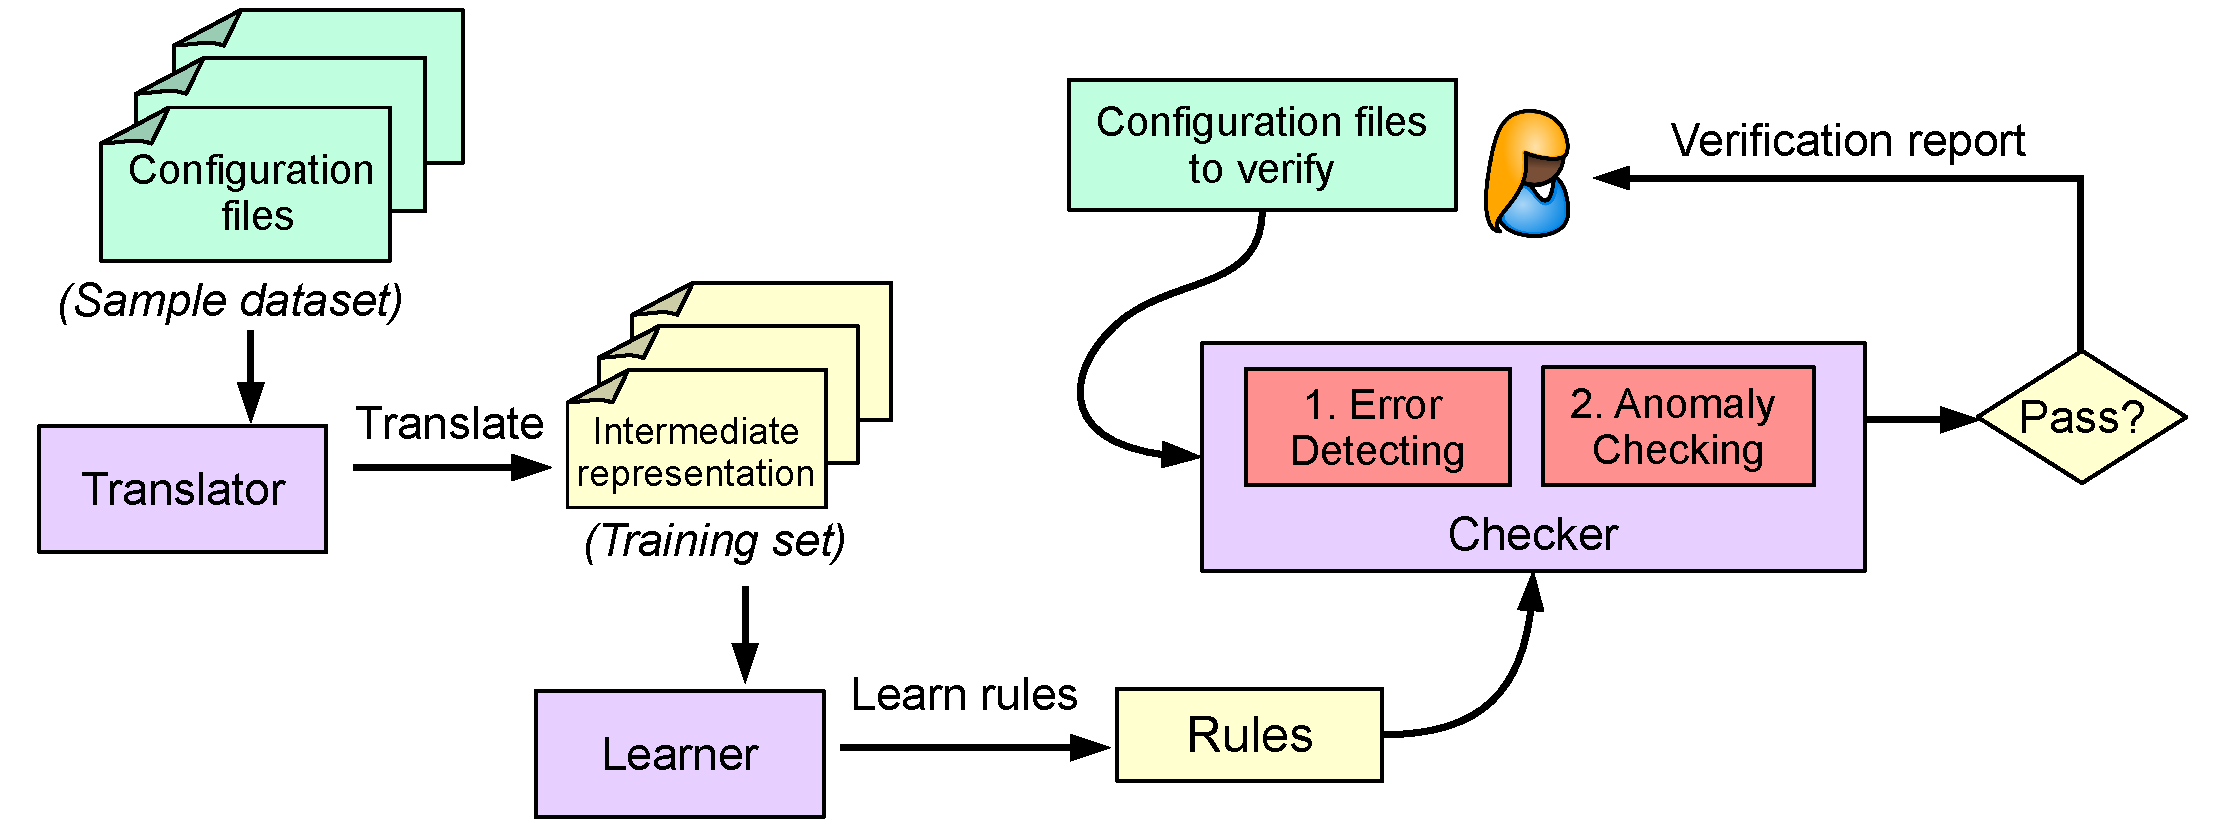
\includegraphics[width=0.88\textwidth]{figs/overview}
\caption{\app's workflow. The green components represent configuration 
  files, including both sample configuration datasets and users' input
  configuration files to verify. 
  The purple components are the modules of \app.
  Because template DB is not necessarily used, we use dashed
  arrow between it and the learner.
  Red boxes are sub-modules within the checker.
  The yellow components are results generated by \app's modules.}
\label{fig-overview}
\end{figure*}

We propose \app, an automatic verification framework,
which can solve configuration errors, \eg, ordering errors
and fine-grained value correlation, that previous work cannot tackle.
As depicted in Figure~\ref{fig-overview}, \app has three main steps:
translation, learning and checking. In this section, we briefly
describe how does each step work.

\para{Initial state.}
We start
with the assumption that we are given a number of (not necessarily) 
correct configuration files belonging to the same system, 
such as MySQL or Apache. 
Such files follow similar patterns, which we exploit
in a learning algorithm to build rules that
describe a language model for the files.

\para{Translator.}
The translator component first parses the input sample 
dataset (containing both configuration files and system environment
information), and then transforms them to a more structured
and typed intermediate representation.
When we run type inference on a configuration file, 
the type of a variable cannot always be fully determined from 
a single value.
We address this problem 
by introducing so called {\em probabilistic types}.
Rather than giving a variable a single type, 
we assign several types with their probability distributions. 
We can later use these more structured files
as a training set to learn the rules. 

\para{Learning.}
The learning algorithm is template-based to be easily extensible. 
We provide an initial set of templates and the
learner learns some concrete instances from the training set. These
rules are used for detecting errors violating the learned constraints
in the files given by the user.

As an illustration of a simple rule that we can learn, consider a template
 $X_1 \le X_2$, where $X_1$ and $X_2$ are
integer variables. The learner might derive the rule stating that
$\texttt{mysql.max\_persistent} \le \texttt{max\_connections}$. There is a classification and taxonomy of configuration errors in the 
existing work on automated configuration troubleshooting~\cite{yin11anempirical, configdataset}. We provide templates for every class that \app can handle: we consider integer constraints, ordering
constraints, typing constraints, and constraints about correlated entries (such as ``if $X$ is present, $Y$ has to appear as well''). 



\subsection{A Language Model for Configuration Files}
\label{sec:lang}

There are several types of configuration 
files and each has different representation. Our goal is to find a good 
intermediary representation that will be language-agnostic. In general,
one can complain that a design of configuration files is pretty low 
level and that we need a new programming language for them. We agree with 
that assertion, and actually our intermediary representation can be seen
as a new programming paradigm for writing configuration files, but this
is not the focus of this proposal. Previously, Huang {\em et al.}~\cite{huang15confvalley} proposed a 
language, ConfValley, to validate 
whether given configuration files meet administrators' specifications. 
However, ConfValley cannot check for misconfiguration checking 
capability, since it is only a library. In ConfValley the administrator 
still needs to write specifications manually, which is an error-prone
process. On the contrary, \app does not require users to manually
write anything.

The translator is a part of \app. It takes as input a sample dataset of configuration files and transforms it into another set of files written in a
typed and well-structured form.
The translator can be seen a parser, and it is
used to translate files into an intermediate representation.

Translating or parsing is system dependent. In other words, for MySQL
and HDFS, we need to develop different parsers to handle each of them,
respectively. Configuration files mainly consists of assignments of the form {\tt {keyword = value}}. Our first attempt was to simply
translate every key-value entry {\tt {k = v}} into a triple $(k, v, \tau)$, where $\tau$ is a type of 
$v$. However, sometimes we could not fully determine the type of key 
based on a single example value. For this reason, we introduced {\emph {probabilistic types}}.

Consider the following example.
\begin{lstlisting}[language=C, xleftmargin=.01\textwidth]
foo = 300
bar = 300.txt
\end{lstlisting} 
Most likely {\tt foo} should be an integer, but it could also be a string.
In the second case, we can learn the rule stating 
$ \texttt{foo} \in \textsf{substrings}(\texttt{bar})$. 
Instead of assigning one type to a value, the translator assigns a distribution of types 
to a value, an idea closely related to existentially quantified 
types~\cite{Launchbury93lazyfunctional}. 

Formally, we define probabilistic types as follows: let $\mathcal{T}$ be a set of basic types (cf. Table~\ref{table:kysymys}).
A probabilistic type built from $\mathcal{T}$ is a list of pairs 
$[(\tau_1, p_1),\ldots,(\tau_n, p_n)]$,
such that $\tau_i \in \mathcal{T}$, $0 \le p_i \le 1$ 
and $\Sigma p_i = 1$. 
These probabilities are updated each time a new example value 
for a key is encountered.

When a value has a probabilistic type, we generate rules for all its types.
This means that by assigning {\texttt{foo}} a probabilistic type 
(\eg, {\tt (\texttt{foo}, 300, [(\textsl{Int},90\%), 
(\textsl{String},10\%)])},
we would generate rules for both strings and integers.
Once the type inference can uniquely determine the type, 
the probability of all other types is set to zero, 
and the associated rules are withdrawn. With the help of probabilistic types, we addressed ambiguities during the parsing phase. 

In \app, the set $\mathcal{T}$ should contains strings, integers, file paths, 
sizes, and IP addresses. With every type, we associate a list of templates 
that are used to learn the rules about those files. Table~\ref{table:kysymys} contains
the most important types and templates.

\begin{table}
\caption{Table of types, along with associated templates, used in \app}
  \begin{tabular}{| l |  l |}
    \hline
    Type &  Template \\ \hline
    \hline
    Integer & $X = Y, X\neq Y, X \leq Y, X < Y, X * Y < Z, \ldots $\\ \hline
    String & $\textsf{substr}(U, V), \textsf{prefix}(U,V), \textsf{suffix}(U,V), \ldots$   \\ \hline
    File Path & $\textsf{isFile}(F), \textsf{isDir}(D),\ldots$   \\ \hline
    Size & Similar to integers   \\ \hline
    Port & $P_1 > P_2$ \\ \hline
    IP Addr.  & $\textsf{sameSubnet}(addr1, addr2)$   \\
    
    \hline
  \end{tabular}
\label{table:kysymys}
\end{table}

In general, the templates works as follows: if there are two entries ${\tt {k1 = v1}}$ and 
${\tt {k2 = v2}}$, and let $t(X, Y)$ be a template that can be applied to those values (w.r.t. their types).
If $t(v1, v2)$ holds, \ie, the template condition is valid for those concrete values, then we will add a rule
$t(k1, k2)$ to a list of potentially correct specifications. Note that the rule expresses a relation between keywords, and not values.

Another problem that we need to address
is that configuration files sometimes contain a simple version of the {\tt {if-then}}, such as in Apache HTTPD, that 
sets conditions for which an action should be applied. Therefore, we also add this guard $g$ to our entry 
during the parsing phase. 

With guards in the picture, when instantiating the rules, we first check
 if the guard is true. If it is not, we simply skip that entry.

To summarize, the translator translates every entry ${\tt {k = v}}$ in a configuration file into a quadruple entry
$$(g,k,v,\textsf{List}[p_1:\tau_1, \ldots, p_n:\tau_n])$$


\section{Learner}
\label{sec-learn}


The goal of the learner module is to derive rules and constraints from
the intermediate representation generated by the translator.
In general, the learner module has two components.
The first component (Sec.~\ref{subsec-rules}) 
learns rules for checking configuration errors like
missing entry errors, ordering errors, 
and fine-grained value correlation errors. 
These errors tend to cause total system failures.
%Once the configuration file has been validated against such rules, 
%the user may choose to invoke a more sensitive constraint checker. 
The second component (Sec.~\ref{subsec-constraints}) aims to derive 
constraints on entries to check for suspicious (or anomalous) values 
that may violate standard practice. These anomalies can cause partial 
degradation of the system, 
such as significant reduction in performance, or even 
total failure~\cite{zhang14encore}.

\subsection{Derivation of ConfigC Rules}
\label{subsec-rules}

The first component is responsible for learning two categories of rules: 
1) rules that are inferred using templates associated with types 
and 2) rules which we call \emph{untyped specifications},
such as ordering or missing entry constraint.
%Both are rules that must hold over multiple parts of a configuration file. 

%However, as mentioned in Sec.~\ref{sec:prelim}, 
%it is difficult to obtain a set of files 
%that is both guaranteed to be without errors
%and large enough to learn sufficiently many rules.
%This usually requires manual verification of the learning set, 
%which is prone to error.
This only considers a rule if it holds over exactly every file in 
the learning set. This behavior can be formally described in Fig~\ref{fig:configC}.

\begin{figure}[!h]
\begin{small}
\belowdisplayskip=-15pt
\abovedisplayskip=-2pt
\begin{align*}
C :=&\ \text{Correct Learning Set}\\
C =&\ \text{\{Configuration Files in Intermediate Representation\}}\\
LR :=&\ \text{Learned Rules} :: \{\textrm{Rule}\}\\
LR =&\ \{ r\ \mid \forall file \in C,\ holds(r,file) \\
&\qquad \ \exists file \in C,\ nontriviallyHolds(r,file)\} 
\end{align*}
\end{small}
\caption{The definition of which rules should be learned by ConfigC}
\label{fig:configC}
\end{figure}

where, the $:: \{Rule\}$ indicates that $LR$ (\ie, the learned rule set) 
is a sets of rules.
The predicate $holds$ indicates that the rule should always be true -
  for instance {\tt max\_connections} $>$ {\tt max\_persistent}.
The predicate $nontriviallyHolds$ indicates that the rule should be true in a meaningful way.
For instance, a file may only contain the keyword {\tt max\_connections} - the previous rule then holds vacuously,
 because we say {\tt max\_connections} is always greater than {\tt max\_persistent} if no value is provided for {\tt max\_persistent} in that file.

\subsection{Derivation of ConfigV Rules}
In \app's learner module, we release the assumption in the above
solution, which means the rule learning mechanism is tolerant 
enough to accept a dataset of possibly incorrect configuration files. 
Rather than manually correcting each file, 
we extend the previous formalism to run probabilistic learning
on our intermediate representations (generated by the translator). 
Our probabilistic approaches for learning missing entry, 
ordering, and fine-grained value correlation rules stem 
from existing work with building 
non-probabilistic versions of these rule-learning algorithms. 
For each of these rules, 
we consider all possible permutations of keys that appear in every 
file which are appropriately typed, and for our learning process, calculate the likelihood that each of 
these permutations constitute a rule. 
Rule patterns in the example set that appear frequently are accepted,
so they can be used to evaluate new files.


\begin{figure}[!h]
\begin{small}
\belowdisplayskip=-15pt
\abovedisplayskip=-2pt
\begin{align*}
U\ :=&\ \text{Unlabeled Learning Set}\\
U =&\ \text{\{Configuration Files in Intermediate Representation\}}\\
LP :=&\ \text{Learned Probabilistic Rules :: \{P\_Rule\}}\\
LR =&\ \{ r\ \mid \Pi file \in C,\ holds(r,file)\ \land \\
&\qquad  \ \Psi file \in C,\ nontriviallyHolds(r,file)\} 
\end{align*}
\end{small}
\caption{The definition of which rules should be learned by ConfigV when learning over a set of possibly correct, and possibly incorrect files.}
\label{fig:configV}
\end{figure}

We use $\Pi$ and $\Psi$ in Fig~\ref{fig:configV} to indicate that the rule holds for some critical portion of the files.
The inuition behind these quantifiers are that we want to consider rules which are true in majority of cases ($\Pi$), 
and for which we have at least some examples for which that rule is nontrivially true ($\Psi$).
The exact definition of $\Pi$ and $\Psi$ is a research question still to be solved.
What exactly is the cutoff value that will yield the best results in learning.
We plan to try multiple strategies to find these values.
One approach may be to use machine learning for program optimization, with a tool like OpenTuner~\cite{ansel:pact:2014}.
It is also possible that this value differs depending on the quality of the learning set and/or the particular type of rule being learned.

\iffalse
Note that the formalism relies on Algorithm~\ref{alg:plearn}. The algorithm considers both typed templates and
untyped specifications. As a similar iteration logic is used for both, an $opt$ flag distinguishes between the two situations.
constructRule in Algorithm~\ref{alg:crules} refers to the creation of a rule from a tuple of entries, 
$m = (e_1, e_2, \ldots, e_i, \ldots, e_{n-1})$.
The rule creation is formally represented as $m(k(e_1), k(e_2), \ldots, k(e_i), \ldots, k(e_{n-1}))$. 
In order to determine if the rule satisfied, the relation associated with $m(v(e_1), v(e_2), \ldots, v(e_i), \ldots, v(e_{n-1}))$ is evaluated for truth.
The rule can be template-generated, for instance {\tt max\_connections} > {\tt mysql.max\_persistent}, or
it can be untyped-specification-generated, for instance the ordering that {\tt recode.so} must come before 
{\tt mysql.so}.

The candidate entry set $Q$ in Algorithm~\ref{alg:plearn} 
differs for the two cases.
For typed templates, due to typing restrictions, 
we must first filter and examine entries associated with the same type, in order to check that 
the template is satisfied over appropriately typed argument entries. This manifests itself via $Q = filter(F,\tau)$
in Algorithm~\ref{alg:plearn}. For
untyped specifications, we do not need to adhere to this typing restriction, so we simply set $Q = F$.

%probability set associated with the rules, $\Pi$, contains values
%ranging from 0 to 1, which are then compared against an acceptance threshold for the final output.
%\[
%\{ P\_Rule = (a_j, a_k) | j \neq k \} \rightarrow \{ (R_1, R_2, ... , R_n) \}
%\]

%We can think of each of these $(a_j, a_k)$ as possibly having a different relationship, defined by the set $\{ R_i \}$, which cover the entire outcome space of possible relationships between the two values $(a_j, a_k)$.

%For the entry missing rules, we define $R_1$ as the event that $a_j$ and
%$a_k$ appear together, and $R_2$ to be the event that $a_j$ appears
%without $a_k$, or by the transitive equivalent, $a_k$ appears without
%$a_j$. For the ordering rules, we define $R_1$ as the event that
%$a_j$ appears before $a_k$ and $R_2$ be the event that $a_k$ appears
%before $a_j$. For the value correlation rules, we define $R_1$ as the
%event that $a_j \leq a_k$, $R_2$ the event that $a_j = a_k$, and $R_3$
%the case that $a_j \geq a_k$. Notice that the $R_i$ do not have to be
%disjoint, but only have to union to the entire probability space.

%By examining the learning set, we will derive a distribution of the set $\{R_i\}$ based on how many times we observe an occurrence of each relation. This distribution will then be used at checking time to determine if a user's configuration has broken a likely rule. 

A rule $r$ will be reported as broken if the probability the rule is
correct, $\Pi(r)$, is greater than some user defined constant, $p$. This
constant can be adjust to the user's preference. A small $p$ will
increase the likelihood of finding an error, but also increase the
number of false positives that are reported.
\fi

\subsection{Learning Suspicious Constraints}
\label{subsec-constraints}

With a configuration file that has been verified against catastrophic
failures (\eg, missing entry, type, and ordering errors), 
the user may also want to examine more subtle issues.
Anomalous values can cause tricky, but impactful, performance and memory
issues that are hard to debug, as discussed in Example 4 of 
$\S$\ref{sec-motiv}. 
Consequently, anomalous values should be flagged and a warning returned
to the user indicating the violation.

We now describe the technique we use to detect anomalous values for 
numerical attributes. Let $A$ be the set of attributes contained in the 
configuration files in the sample dataset. 
Let $A_n$ be the subset of attributes of $A$ which are numerically typed. 
Then, for each attribute $a \in A_n$, we construct a vector $v_a$ of the 
values corresponding to attribute $a$, seen over the entire sample dataset.
For each $v_a$, we compute 
an interval  $$[\hat{v_a} - 50*MAD(v_a), \hat{v_a} + 50*MAD(v_a)],$$ 
where $\hat{v_a}$ represents the median over the values 
in $v_a$ and $MAD(v_a$) refers to the 
median absolute deviation. 
This is a variant of a standard outlier detection test, namely the Hampel identifier.\footnote{Mathematically, $MAD(v_a) = 1.4826* median(|v_a - \hat{v_a}|)$, estimating standard deviation 
for a normal distribution.} 
In the checking phase, as long as the checker finds a value for a numerical 
attribute in the checked file outside of this interval, 
a warning would be printed to the user indicating the violating value, 
the attribute, and the upper or lower Hampel threshold. 

The intuition behind this is that if the user has input a value 
that falls outside of an interval containing values that are considered 
``normal'' over the entire sample dataset, 
that value will probably cause an error, in particular for performance. 
We cannot know for sure if this value will cause an issue. 
For instance, a user might have a machine with 
particularly high-end hardware, 
in which case a value beyond the upper Hampel threshold may be appropriate. 


\section{Extending \app and Applying it to Real-World Configurations}
\label{sec:travis}

TravisCI~\cite{API} is a popular integration and build testing service 
connected to Github. It has been used on more than 17 
millions of projects. 
TravisCI allows programmers to automatically run their test suite on a fresh virtual machine every time they commit their code.
A TravisCI user must add a configuration file to the repository that specifies build conditions, 
such as which dependencies are required, and a set of benchmarks to test. 
The results of these tests (indicating either passing, failing, or misconfiguration) 
are saved by TravisCI on a publicly available database~\cite{API}.

TravisCI misconfigurations are important to detect and correct before execution,
because any failed compilation can costs developer significant amount 
of time. A misconfiguration can cause a test suite to run up to 20 
minutes, only to report that the whole computation failed~\cite{API}.
If developer would have this information prior to the compilation attempt, they could
 identifying and correct potential misconfigurations.

A new challenge here is that we need to reason about a 
temporal component too. Having an entire TravisCI log for a given
project we can examine the sequence of changes of a configuration file
and we can detect what has changed so that we switched from a failing 
compilation to successful compilation. 

%Driven by the above motivating example, we propose an extension to \app that
%learns over a training set with both correct and incorrect examples, as well as a temporal structure.
%Such an extension employs an existing technique from the machine learning community, called version space learning,
%to significantly decrease the false positive rate while maintaining the detection capability of \app.

\subsection{Version Space Learning with Temporal Properties} 

We plan to use version space learning and SMT solvers to detect errors in 
TravisCI configurations files. Version space learning 
builds a logical constraint model for binary
classification~\cite{mitchell77}, which we use to test a configuration file for 
membership in the set of all correct files.

\begin{wrapfigure}{l}{0.5\textwidth}
  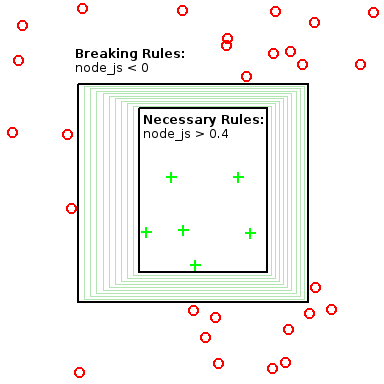
\includegraphics[width=0.45\textwidth]{figs/Version_space}
  \caption{\small Red circles are failing files, and green pluses are passing files.}
  \label{fig:versionSL}
\end{wrapfigure}

Figure~\ref{fig:versionSL} outlines our proposed approach. We first apply the standard ConfigC approach to learn the rules that have 
to hold for correct TravisCI configuration files. Traditionally, 
version space learning builds a model that defines membership using a series of 
disjunctions from a set of predefined hypotheses.  However, we need  to 
use conjunctions to convey that a configuration file is only correct if 
it satisfies all the learned relations. Those rules can be seen as
positive examples in classifying correct files. In addition, we will have
so-called {\emph {breaking rules}} which are derived from the files 
that do not compile, \ie~negative examples. Breaking rules are specified 
using disjunctions.

Figure~\ref{fig:versionSL} shows an example set of necessary and breaking rules that would be learned if the training set contains a failing file indicating that 
{\small node\_js} version is 0.2, and a passing file has its version set to 0.4.
With red dots we depict incorrect files that do not compile, and the green crosses show correct files.
From both types of files, we extract breaking and necessary rules, which define borders between those two sets of files.
This results in a space (green stripes) where a file may contain relations that cannot be classified as either breaking or necessary.
For example, if a user provides a file which specifies version 0.3 of {\small node\_js}, this file will fall in the green striped space.
Part of the research task will be to find an optimal classification for such cases.

The success or failure of a TravisCI configuration file is dependent
not only on the configuration file itself (namely, a .travis.yml file) but it also depends on system information such as programming languages and a list of imported libraries.
For this reason, we call this extended configuration files a program summary, denoted with $P_t$. This is a representation 
of the repository which contains any information 
relevant to the learning process.
The subscript on $P_t$ is a timestamp tag based on 
the ordered git commit history.
%In the case of TravisCI, this include the \verb|.travis.yml| file, 
%as well as code features that may effect build status, 
%such as programming language and a list of imported libraries.
%The summary must be \textit{sufficiently detailed}, that is it must contain every piece of information that might lead to a build error.

%IMPORTANT, but no space
%However, a git history is not a limited to a single linear timeline.
%Git features the ability to \textit{branch}, which allows to simultaneous commit chains.
%To handle the start of a branch, add a superscript to indicate the branch, and restart the counter on a branch.
%To handle the merge of two branches $P_{t}^{x}$ and $P_{t'}^{y}$, step to $P_{t+1}^{x}$, where $x$ is the mainline branch.
%We then say that $P_{t'}^{y}$ has no successor commit $P_{t'+1}^{y}$.

From these summaries we will build a model $M(P_t)$, using the same techniques as in 
\app. $M(P_t)$ actually is a set of all possible relations derivable 
from the program summary. As previously, we need to construct templates for the 
learning process, since the level of specification details depends on them.

We now outline how we plan to use SMT solvers to find the sets of necessary rules ($Nec$), and the set of breaking rules ($Br$).

Let $S(P_t)$ be the build status returned from TravisCI when run on $P_t$.
It can be either $Pass$ or $Err$. We define shorthand $S(P_{t,t+1}) = PE$ to 
state that the program was compiling before and now it does not:
\begin{align*}
  S(P_{t,t+1}) = PE :\Leftrightarrow S(P_t)=Pass \land S(P_{t+1})=Err 
\end{align*}

We now consider both incorrect and correct files in the training set 
and so must introduce the \textit{general boundary}.
The general boundary is the dual of the specific boundary, and is the most relaxed requirement for a positive classification.
We denoted specific boundary as the set of necessary relations $Nec$, and now denote the general boundary as the set of breaking relations $Br$.
With this notation, we can formally express the requirement that the program summary is sufficiently detailed.
\begin{align}
  \forall S(P_t)=Err, \exists r \in M(P_t), r \in Br \label{eq:E1}
\end{align}

From the above we know that if a build is erroring, then there must exist at least one error.
We can also know that if a build is passing, then there must not exist any errors.
That is, the model of a passing commit must not contain any rules which are breaking.
Note we are not, however, guaranteed that any rules from a passing commit are necessary.
\begin{align}
  S(P_t) = Err \implies \exists r \in  M (P_t), r \in Br \label{eq:E}\\
  S(P_t) = Pass \implies \forall r \in  M (P_t), r \notin Br \label{eq:P}
\end{align}

%While Eq. \ref{eq:E} and \ref{eq:P} might build a basic model, they will do not capture all of the available knowledge.
%The key insight is that 
Additionally, when we commit a break ($PE$), we can localize the error to one of the relations that changed.
Either we removed something that was necessary, or added something that was breaking.
Note that this is an inclusive disjunction, since a erroring commit can break multiple things at once.
Expressed formally, where $\setminus$ is the set difference, that is:
\begin{align}
  S(P_{t,t+1}) &= PE \implies \nonumber \\
  \exists& r \in (M(P_{t})\ \setminus M(P_{t+1})), r \in Nec\ \nonumber \\
  \lor \ \exists& r \in (M(P_{t+1}) \setminus M(P_{t})), r \in Br \label{eq:PE}
\end{align}

We then can combine \eqref{eq:E}, \eqref{eq:P}, and  \eqref{eq:PE} with
conjunctions and ask a SMT solver for a model satisfying the formula.
The resulting model will be the sets of necessary rules ($Nec$), and the set of breaking rules ($Br$), which can be used to check new configuration files.
Since we used a similar model to \app, we will still be able to provide justifications for the classification results.



\section{Related Work}

\iffalse
Configuration verification has been considered a promising way  
to tackle misconfiguration problems~\cite{xu15systems}.
Nevertheless, a practical and automatic configuration
verification approach still remains an open problem.

\para{Language-support misconfiguration checking}
There have been several language-support efforts proposed for preventing
configuration errors introduced by fundamental deficiencies in
either untyped or low-level languages. For example, in the network
configuration management area, administrators often
produce configuration errors in their routing configuration files.
PRESTO~\cite{enck07configuration} 
automates the generation of device-native configurations
with configlets in a template language. 
Loo {\em et al.}~\cite{loo05declarative} adopt Datalog to reason about 
routing protocols in a declarative fashion. 
COOLAID~\cite{chen10declarative} constructs
a language to describe domain knowledge about devices and
services for convenient network reasoning and management.
Compared with the above efforts, our work focuses on software systems, 
\eg, MySQL and Apache, and our main purpose is to automate configuration
verification rather than proposing new languages 
to convenient configuration-file writing. 

\para{Misconfiguration detection}
Misconfiguration detection techniques aim at checking configuration
efforts before system outages occur.
Most existing detection approaches check 
the configuration files against a set of predefined correctness 
rules, named constraints, and then report errors if 
the checked configuration files do not satisfy these rules.
Huang {\em et al.}~\cite{huang15confvalley},
for example, proposed a 
language, ConfValley, to validate 
whether given configuration files meet administrators' specifications. 
As opposed to our work, ConfValley does not
have inherent misconfiguration checking capability, since it only offers
a language representation and requires administrators to
manually write specifications, which is an error-prone
process. On the contrary, our work does not need users to manually
write anything.

Several machine learning-based misconfiguration detection efforts 
also have been proposed~\cite{yuan11context, zhang14encore, xu16early}.
EnCore~\cite{zhang14encore} introduces a template-based
learning approach to improve the accuracy of their learning results.
The learning process is guided by a set of predefined rule templates
that enforce learning to focus on patterns of interest.
In this way, EnCore filters out irrelevant information and reduces
false positives; moreover, the templates are able to express
system environment information that other machine learning
techniques cannot handle.
Compared with EnCore, \app has the following advantages.
First, \app does not rely on any template. 
Second, EnCore cannot detect missing entry errors, type errors,
ordering errors and fine-grained integer correlation errors,
but \app can detect all of them.
Finally, \app is a very automatic system, but
EnCore needs significant human interventions, \eg, system parameters
and templates.

PCheck~\cite{xu16early} aims to add configuration checking code to the system source code by emulating potential commands and behaviors of the system. 
This emulation is a ``white-box'' approach and requires access to the system's source code.
One drawback to this approach is that for some systems (\eg, ZooKeeper) whose behavior is 
hard to emulate, PCheck cannot automatically generate the corresponding checking code.
Due to the emulation based testing strategy, PCheck's scope is limited to reliability problems caused by misconfiguration parameters. 
In contrast, \app is a ``black-box'' approach and only requires a training set of configuration files to learn rules.
By using a rule learning strategy of examples, \app is able to detect general misconfiguration issues that are outside the scope of emulation testing (\eg memory or thread usage settings), including performance, security, availability and reliability.

\para{Misconfiguration diagnosis}
Misconfiguration diagnosis approaches have been proposed to address configuration problems post-mortem.
For example, ConfAid~\cite{attariyan10automating} 
and X-ray~\cite{attariyan12x-ray} use dynamic information
flow tracking to find possible configuration errors that may have resulted in
failures or performance problems. AutoBash~\cite{su07autobash} 
tracks causality and automatically fixes 
misconfigurations. Unlike \app, most misconfiguration
diagnosis efforts aim at finding errors after system
failures occur, which leads to prolonged recovery time.

\fi

\newpage

\setcounter{page}{1}
\bibliographystyle{plain}
\bibliography{os}

\end{document}
